% ============================ ATTACCHI E SICUREZZA SU AES ===============================

\chapter{Attacchi e Sicurezza su AES} %TODO: rename in Attacchi e Sicurezza di AES?

%TODO: Pros e Cons (Tipi Attacchi su AES, vulnerabilità?, ecc.) %TODO: volendo resistance to linear and differential cryptoanalysis, wide tail strategy, impractical related key attacks.

%TODO: Man in the middle?
%TODO: Template Attack?

% ========================================================================================

% ---------------------------- SECTION: INTRODUZIONE --------------------------------------

\section{Introduzione}

\textsf{\small In questo capitolo, verranno brevemente trattati i possibili attacchi e la sicurezza in generale di AES come cifrario.}

% ------------------------------- SECTION: ATTACCHI --------------------------------------

\section{Attacchi}

\textsf{\small }

\subsection{CCA | No Chosen Ciphertext Attack}

\textsf{\small Questo è un tipo di attacco in cui l'attaccante è a conoscenza sia del testo cifrato che di quello decifrato. Riesce a ottenere la decifrazione del testo cifrato attraverso il recupero di informazioni che permettono questo di ottenere la chiave segreta.}

%TODO: È possibile in una modalità come ECB?/.

%TODO: Immagine?

\subsection{Sample Tampering Attack}

\textsf{\small }

\subsection{Side Channel Attack}

\textsf{\small Questi sono tipi di attacchi che sfruttano ogni minima informazione ottenuta, non da difetti nell'algoritmo in sé per sé, ma nel modo in cui questo è stato implementato. Alcune di questi tipi di informazioni che si potrebbero ottenere sono informazioni sul tempo di esecuzione, consumo di energia elettrica, perdita di radiazioni elettromagnetiche e suoni.}

\begin{figure}[H]
	\centering
	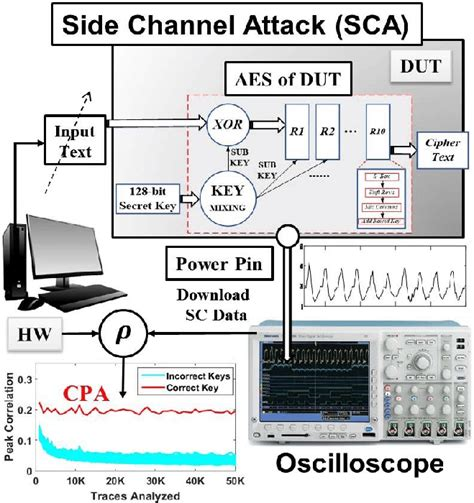
\includegraphics[width=.6\textwidth, height=.6\textheight, keepaspectratio]{./images/attacks/side_channel_attack.png}
	\caption{Attacco dal canale laterale}
	\label{fig:side_channel_attack}
\end{figure}

\subsection{MITM | Meet-In-The-Middle}

\textsf{\small Questo genere di attacco, da non confondere col \emph{man-in-the-middle}, è basato su una vulnerabilità di spazio-tempo di un algoritmo crittografico che esegue diverse operazioni di cifratura in sequenza.}

\subsection{Biclique Attack}

\textsf{\small L'attacco \emph{biclique} è un particolare tipo di attacco \emph{MITM} (Meet-In-The-Middle) che utilizza un \emph{biclique} (grafo bipartito completo) per estendere il numero possibile di rounds di attacchi dell'attacco MITM.}

\subsection{Related Key Attacks}

\textsf{\small L'attacco delle chiavi correlate è un attacco in cui l'attaccante attraverso l'osservazione di varie chiavi, i cui valori sono sconosciuti inizialmente, riesce a ricavarne qualche relazione matematica tra queste.} %TODO: rimuovere tra queste?

\subsection{Social Engineering}

\textsf{\small L'attacco di tipo \emph{ingegneria sociale} è un attacco che riguarda la manipolazione psicologica delle persone per poter ottenere informazioni confidenziali.}

\subsection{Fault Attacks}

\textsf{\small Questi tipi di attacchi cercano di trarre vantaggio di difetti accidentali o fatti apposta iniettati durante la computazione dell'algoritmo. Riguardo ad AES, sono possibili attacchi di questo tipo in grado di ridurre la grandezza della chiave a $2^8$ con una complessità di $2^{30}$ e anche attacchi sulla \emph{key expansion}.}

\subsection{Cache-Timing Attacks}

\textsf{\small Questa classe di attacchi in cui l'attaccante tenta di compromettere il sistema crittografico analizzando il tempo di esecuzione dell'algoritmo. Prendono vantaggio degli intervalli di tempo tra la cache e gli accessi alla memoria principale.}

\subsection{Attacks on Reduced-Round AES}

\textsf{\small È possibile che con un ridotto numero di rounds, AES è vulnerabile. È stato scoperto, in fase di progettazione che era possibile trovare una scorciatoia con AES con 6 rounds, per questo ne sono stati aggiunti altri 4. È stato possibile recuperare la chiave con un AES fornito di soli 5 rounds.}

\subsection{PA | Padding Attack}

\textsf{\small Un attacco di padding si basa sul fatto che un messaggio deve essere di una determinata lunghezza per poter essere compatibile alla grandezza della primitiva crittografica, grandezza del blocco per AES. L'attacco conta sul conoscere se al messaggio è stato aggiunto il padding in modo corretto o no.}

\textsf{\small Alcune modalità che potrebbero soffrire di questo tipo di attacco sono CBC OAEP (Optimal Asymmetric Encryption Padding).} %TODO: rimuovere OAEP?

% ------------------------------- SECTION: SICUREZZA --------------------------------------

\section{Sicurezza}

\textsf{\small }

%TODO: In generale la sicurezza di AES

% ============================ FINE CAPITOLO ==============================================